
%%%%%%%%%%%%%%%%                                ~~~~~~~~~~~~~~~~~~~~~~~~~~~~~~~~~~~~~~~~~~~~~~~~~~
% CONDITIONALS %
%%%%%%%%%%%%%%%%                                ~~~~~~~~~~~~~~~~~~~~~~~~~~~~~~~~~~~~~~~~~~~~~~~~~~

\newif\ifPeerReview\PeerReviewfalse              % Whether to create the PeerReview version or
                                                % Journal version
\newif\ifOnlineColor\OnlineColortrue            % Compile online color version?

\newif\ifFlatArchive\FlatArchivefalse           % Whether archive is flat (messy) or contain 
                                                % subfolders for graphics etc.
\newif\ifFloatAtEnd\FloatAtEndfalse             % Available in PeerReview mode:
                                                % Place floats at end of document?
\newif\ifTODO\TODOtrue                        % Use todo notes?

\ifOnlineColor
   \newcommand\figPostfix{_online}              % Colored images online
\else
   \newcommand\figPostfix{_bw}                  % Black and white in journal
\fi

%%%%%%%%%%%%                                    ~~~~~~~~~~~~~~~~~~~~~~~~~~~~~~~~~~~~~~~~~~~~~~~~~~
% IEEEtran %
%%%%%%%%%%%%                                    ~~~~~~~~~~~~~~~~~~~~~~~~~~~~~~~~~~~~~~~~~~~~~~~~~~

\ifPeerReview
\documentclass[10pt,journal,draftclsnofoot,onecolumn]{IEEEtran}
% \newcommand\CLASSINPUTbaselinestretch{1.66}     % http://theoval.cmp.uea.ac.uk/~nlct/latex/thesis/node17.html
\else
\documentclass[journal]{IEEEtran}
\fi

% \RequirePackage[latin1]{inputenc}%              % Set input encoding (optionally latin1)
% \RequirePackage[T1]{fontenc}%                 % Set font encoding
% \usepackage[norsk]{babel}

% Single column review mode:
%\documentclass[12pt,journal,onecolumn]{IEEEtran}
%\newcommand\CLASSINPUTbaselinestretch{2}
%\RequirePackage{calc}
%\RequirePackage{fp} 
% Left margin = 1 inch + hoffset + oddsidemargin (or evensidemargin)
% Adding the 2cm gutter width to the odd/even side margins:
%\setlength\hoffset{0pt}
%\setlength\oddsidemargin{4cm}       % 4cm margins on the left side
%\addtolength\oddsidemargin{-1in}    % Subtract the initial 1 inch
%\setlength\textwidth{21cm-8cm}    % A4 width (21cm) minus margins on either side

%%%%%%%%%%%%%%%%%%%%%%%%%%%%%%                  ~~~~~~~~~~~~~~~~~~~~~~~~~~~~~~~~~~~~~~~~~~~~~~~~~~
% IEEE ''APPROVED'' PACKAGES %
%%%%%%%%%%%%%%%%%%%%%%%%%%%%%%                  ~~~~~~~~~~~~~~~~~~~~~~~~~~~~~~~~~~~~~~~~~~~~~~~~~~

\usepackage{cite}

\ifCLASSINFOpdf
   \usepackage[dvips]{graphicx}                 % Might not work. Use 'latex' instead of 
   \ifFlatArchive\else                          % 'pdflatex'
      \graphicspath{./gfx/}
   \fi
\else
   \usepackage[dvips]{graphicx}
   \ifFlatArchive\else
      \graphicspath{./gfx/}
   \fi
\fi

\RequirePackage[table,dvipsnames,svgnames]{xcolor}

\usepackage[cmex10]{amsmath}                    % cmex10 option to be IEEE explore compliant
\interdisplaylinepenalty=2500                   % Allows multiline equations to be broken

% \RequirePackage{amssymb}

\RequirePackage{array}

\ifCLASSOPTIONcompsoc
   \usepackage[caption=false,font=normalsize,labelfont=sf,textfont=sf]{subfig}
\else
   \usepackage[caption=false,font=footnotesize]{subfig}
\fi

% \usepackage{caption}
% \usepackage{subcaption}
\usepackage{color}
\usepackage{calc}
\usepackage{fp}

% 
% \ifCLASSOPTIONcaptionsoff                       % IEEE promoted hack to turn off captions from the 
%    \let\MYorigsubfloat\subfloat                 % subfloat package should the captionsoff option
%    \renewcommand{\subfloat}[2][\relax]{\MYorigsubfloat[]{#2}} % be specified.
% \fi

\ifFloatAtEnd
\ifCLASSOPTIONcaptionsoff                       % Places float at the end of the document when the
  \usepackage[nomarkers]{endfloat}              % captionsoff options is specified to IEEEtrans.cls
  \let\MYoriglatexcaption\caption               % (PeerReview mode)
  \renewcommand{\caption}[2][\relax]{\MYoriglatexcaption[#2]{#2}}
\fi
\fi

\usepackage{fixltx2e}                           % Fix some twocolumn float problems

\usepackage{stfloats}                          % Allows: \begin{figure*}[!b]
                                                % (double column figures on top/bottom)

\usepackage{url}                                % Support for handling and breaking URLs

% NOTE: PDF hyperlink and bookmark features are not required in IEEE
%       papers and their use requires extra complexity and work.
\newcommand\MYhyperrefoptions{bookmarks=true,bookmarksnumbered=true,
pdfpagemode={UseOutlines},plainpages=false,pdfpagelabels=true,
colorlinks=true,linkcolor={black},citecolor={black},urlcolor={black},
pdftitle={A Fast GPU Sonar Simulator for Automatic Target Recognition},
pdfsubject={},
pdfauthor={Jo Inge Buskenes},
pdfkeywords={adaptive beamforming, beamforming, complexity, sonar, active}}%
\ifCLASSINFOpdf
   \usepackage[\MYhyperrefoptions,pdftex]{hyperref}
\else
   \usepackage[\MYhyperrefoptions,breaklinks=true,dvips]{hyperref}
   \usepackage{breakurl}                        % Allows 'dvips' driver to break links
\fi

%%%%%%%%%%%%%%%%%%%%%%%                         ~~~~~~~~~~~~~~~~~~~~~~~~~~~~~~~~~~~~~~~~~~~~~~~~~~
% ADDITIONAL PACKAGES %       
%%%%%%%%%%%%%%%%%%%%%%%                         ~~~~~~~~~~~~~~~~~~~~~~~~~~~~~~~~~~~~~~~~~~~~~~~~~~

% \ifPeerReview
% \let\OldIncludegraphics{\includegraphics}
% \usepackage{letltxmacro}
% \LetLtxMacro{\OldIncludegrsaphics}{\includegraphics}
% \renewcommand{\includegraphics}[2][]{\OldIncludegraphics[width=\linewidth, #1]{#2}}
% \fi

% % \makeatletter
% % \def\maxwidth{\ifdim\Gin@nat@width>\linewidth\linewidth
% % \else\Gin@nat@width\fi}
% % \makeatother
% % \let\Oldincludegraphics\includegraphics
% % \renewcommand{\includegraphics}[1]{\Oldincludegraphics[width=\maxwidth]{#1}}

\usepackage[maxfloats=40]{morefloats}
\newcounter{todoidx}
% \setcounter{todoidx}

\ifTODO
   \definecolor{todobackground}{rgb}{0.95,0.95,0.95}
   \setlength\marginparsep{1pt}
   \setlength\marginparwidth{35pt}
   \newlength\marginparwidthsmall
   \setlength\marginparwidthsmall{\marginparwidth}
   \addtolength\marginparwidthsmall{-7pt}
   \newcommand\todo[1]{%
      \addtocounter{todoidx}{1}%
      {\color{Red}\bf(\thetodoidx{})}%%\fbox{\bf\thetodoidx{}}}%
      \marginpar{%
         {\vspace*{-10pt}\color{Red}\fbox{\bf\thetodoidx{}}}\\%
         \fcolorbox{red}{todobackground}{\parbox{\marginparwidthsmall}{\scriptsize #1}}}}

   \newcommand\todopar[1]{\fcolorbox{red}{white}{\parbox{0.97\linewidth}{#1}}}
\else
%    \usepackage[disable]{./todonotes} 
   \newcommand\todo[1]{}
\fi

\newenvironment{narrow}[2]{%
\begin{list}{}{%
\setlength{\topsep}{0pt}%
\setlength{\leftmargin}{#1}%
\setlength{\rightmargin}{#2}%
\setlength{\listparindent}{\parindent}%
\setlength{\itemindent}{\parindent}%
\setlength{\parsep}{\parskip}}%
\item[]}{\end{list}}

\usepackage{float}

\ifOnlineColor
   \definecolor{tabBlue}{HTML}{AACCFF}
\else
   \definecolor{tabBlue}{HTML}{CCCCCC}
\fi

%%%%%%%%%%                                      ~~~~~~~~~~~~~~~~~~~~~~~~~~~~~~~~~~~~~~~~~~~~~~~~~~
% MACROS %       
%%%%%%%%%%                                      ~~~~~~~~~~~~~~~~~~~~~~~~~~~~~~~~~~~~~~~~~~~~~~~~~~

\newcommand\graphicsAI[2][]{%
  \immediate\write18{./bin/laFigure #2 #1}%
  \input{result}}%
  
% \DeclareMathOperator*{\argmin}{\text{arg}\;\text{min}}

\newcommand\Fig[1]{Fig.~\ref{#1}}

\newcommand\Grey[1]{{\color{Grey}#1}}
\newcommand\Red[1]{{\color{Red}#1}}
\newcommand\Blue[1]{{\color{Blue}#1}}
\newcommand\DarkBlue[1]{{\color{DarkBlue}#1}}
\newcommand\LightBlue[1]{{\color{LightBlue}#1}}
\newcommand\Brown[1]{{\color{Brown}#1}}
\newcommand\Green[1]{{\color{Green}#1}}
\newcommand\SeaGreen[1]{{\color{SeaGreen}#1}}
\newcommand\Yellow[1]{{\color{yellow}#1}}
\newcommand\Orange[1]{{\color{orange}#1}}

\newcommand\nn{\nonumber\\}

\newcommand\nmat[1]{\begin{matrix}#1\end{matrix}}
\newcommand\bmat[1]{\begin{bmatrix}#1\end{bmatrix}}
\newcommand\case[1]{\begin{cases}#1\end{cases}}
\newcommand\textbox[2]{\footnotesize\text{\parbox{#1}{\centering\emph{#2}}}}

\newcommand\rand{\text{rand}}
\newcommand\randn{\text{randn}}
\newcommand\rect{\text{rect}}
\newcommand\sinc{\text{sinc}}
\newcommand\tr{\text{tr}}
\newcommand\adj{\text{adj}}

% \newcommand\max{\text{max}}
\newcommand\argmin[1]{\text{arg}\;\underset{#1}{\text{min}}}

\newcommand\qqquad{\quad\qquad}
\newcommand\qqqquad{\qquad\qquad}

% \renewcommand\l[1]{\left#1}
% \renewcommand\r[1]{\right#1}

% {\text{\parbox{1.5cm}{\centering volume hyper- sphere}}}

%Keyword colouring:
\newcommand\kw[1]{#1}
\newcommand\parm[1]{#1}%\color{Black}#1\color{Black}}

\newcommand\of[1]{\scriptstyle(\parm{#1})\displaystyle}
\newcommand\df[1]{\scriptstyle[\parm{#1}]\displaystyle}
\newcommand\var[3]{#1_\text{#2}\of{#3}}

\newcommand\diag{\text{diag}}

% \raisebox{lift}[extend-above-baseline][extend-below-baseline]{text}
\newcommand\mt[1]{\text{\emph{#1}}} %mt = mathtext
\newcommand\mathnorm{\textstyle}
\newcommand\mathbig[1]{\displaystyle#1\mathnorm}
\newcommand\mathsmall[1]{\scriptstyle#1\mathnorm}
\newcommand\mathtiny[1]{\scriptscriptstyle#1\mathnorm}
\newcommand\sfrac[2]{\scriptstyle\raisebox{0.25pt}[0pt][0pt]{$\frac{#1}{#2}$}\mathnorm}
\newcommand\nfrac[2]{\textstyle\frac{#1}{#2}\displaystyle}

\newcommand\sumu[1]{\sum\limits^{#1}\;}
\newcommand\suml[1]{\sum\limits_{#1}\;}
\newcommand\sumb[2]{\sum\limits_{#1}^{#2}\;}

\newcommand\produ[1]{\prod\limits^{#1}\;}
\newcommand\prodl[1]{\prod\limits_{#1}\;}
\newcommand\prodb[2]{\prod\limits_{#1}^{#2}\;}

\newcommand\defeq{\overset{\underset{\mathrm{def}}{}}{=}}

%Math macros:
\newcommand\T{^{\scriptscriptstyle T}}
\renewcommand\H{^{\scriptscriptstyle H}}

\renewcommand\vec[1]{\boldsymbol{#1}}
\newcommand\mat[1]{\boldsymbol{#1}}

\newcommand\Om{O_\text{m}}
\newcommand\Oa{O_\text{a}}
\newcommand\Nl{N_\text{l}}
\newcommand\Nk{N_\text{k}}
\newcommand\1{\vec 1}
\newcommand\I{\mat I}
\renewcommand*\a{\vec a}
\renewcommand*\i{\vec i}
\renewcommand*\k{\vec k}
\newcommand*\n{\vec n}
\newcommand*\p{\vec p}
\newcommand*\s{\vec s}
\newcommand*\w{\vec w}
\newcommand*\x{\vec x}
\newcommand*\y{\vec y}

\newcommand*\A{\mat A}
\newcommand*\B{\mat B}
\newcommand*\C{\mat C}
\newcommand*\E{\mat E}
\renewcommand*\P{\mat P}
\newcommand*\eP{\mat{\hat P}}
\newcommand*\R{\mat R}
\newcommand*\Ri{\R^{-1}}
\newcommand*\eR{\mat{\hat R}}
\newcommand*\eRi{\hat{\mat R}\;\!^{-1}}
\newcommand*\Navg{N_\text{avg}}
\newcommand*\W{\mat W}
\newcommand*\X{\mat X}
\newcommand*\Xd{\X_{\!\Delta}}
\newcommand*\Y{\mat Y}


\renewcommand*\P{\mat P}
\newcommand*\V{\mat V}
\newcommand*\M{\mat M}

\renewcommand*\L{\mat \Lambda}
\newcommand*\U{\mat U}
% \renewcommand*\t{\mathtiny{^T}}
% \newcommand*\h{\mathtiny{^H}}
\renewcommand*\t{^T}
\newcommand*\h{^H}

\usepackage{tikz}
\usetikzlibrary{shapes,snakes}
\usepackage{amsmath,amssymb}
% \usepackage{datatool}
% \usepackage{glossaries}

\newenvironment{outline}
{\begin{itemize}}
{\end{itemize}}


% correct bad hyphenation here
% \hyphenation{op-tical net-works semi-conduc-tor}

%%%%%%%%%%%%                                    ~~~~~~~~~~~~~~~~~~~~~~~~~~~~~~~~~~~~~~~~~~~~~~~~~~
% GLOSSARY %
%%%%%%%%%%%%                                    ~~~~~~~~~~~~~~~~~~~~~~~~~~~~~~~~~~~~~~~~~~~~~~~~~~

% \makeglossaries
% \newglossaryentry{ASIC}{name={ASIC},
                  description={Application Specific Integrated Circuit} } 
                  
\newglossaryentry{ATR}{name={ATR},
                  description={Automatic Target Recognition} } 

\newglossaryentry{CPU}{name={CPU},
						description={Central Processing Unit} } 

\newglossaryentry{GPGPU}{name={GPGPU},
						description={General Purpose Graphics Processing Unit} } 

\newglossaryentry{GPU}{name={GPU},
						description={Graphics Processing Unit} } 
					
\newglossaryentry{MVDR}{name={MVDR},
						description={Minimum Variance Distortionless Response} } 

%%%%%%%%%%%%%%%%%%                              ~~~~~~~~~~~~~~~~~~~~~~~~~~~~~~~~~~~~~~~~~~~~~~~~~~
% DOCUMENT START %
%%%%%%%%%%%%%%%%%%                              ~~~~~~~~~~~~~~~~~~~~~~~~~~~~~~~~~~~~~~~~~~~~~~~~~~

% \usepackage{yfonts}

% \graphicspath{submission/final/gfx/}

\begin{document}


\title{A Real-Time Sonar Simulator for Automatic Target Recognition}

\author{{Jo~Inge~Buskenes,~\IEEEmembership{Student Member,~IEEE,} %
        Herman~Midelfart, %
        \O{}ivind~Midtgaard} %
\thanks{J. I. Buskenes is with the Department of Informatics, University of Oslo, Norway.}%
\thanks{H. Midelfart and \O. Midtgaard are with The Norwegian Defence Research Establishment (FFI), Norway.}% <-this % stops a space
% \thanks{Manuscript received April 19, 2005; revised January 11, 2007.}
}

% The paper headers
\markboth{IEEE Journal of Oceanic Engineering}%
{A GPU Sonar Simulator for Automatic Target Recognition}

% Publishers ID mark:
%\IEEEpubid{0000--0000/00\$00.00~\copyright~2007 IEEE}

% use for special paper notices
%\IEEEspecialpapernotice{(Invited Paper)}

% for Computer Society papers, we must declare the abstract and index terms
% PRIOR to the title within the \IEEEcompsoctitleabstractindextext IEEEtran
% command as these need to go into the title area created by \maketitle.
\IEEEcompsoctitleabstractindextext{%
\begin{abstract}
Template matching is a common technique for automatic classification of objects in synthetic aperture sonar (SAS) images. The principle is to isolate an image segment containing the object of interest, correlate it with a set of template images, and assign it to the class of the template yielding the highest correlation coefficient. The challenge is to come up with a representative set of template images covering the relevant configurations of object and seabed.

We target this challenge with a sonar simulator that first takes as input a seabed model derived from the real sonar image. Then it places a 3D object model on the seabed, renders the scene, and adds the resulting image to the template set. For every object type, position, alignment and material, the procedure is repeated, and a correlation coefficient computed. The best performance is obtained when these parameters are estimated from the sonar image as part of the classification process. The simulator is therefore written in OpenGL and OpenCL and runs on graphics processing units (GPUs). The result is a fast performing and portable template generator which can adapt to the characteristics of the current scene on-the-fly.
\end{abstract}

% Keywords (normally not used for peer reviews)
\ifPeerReview\else
\begin{IEEEkeywords}
Sonar, SAS, simulator, template matching, OpenGL, OpenCL.
\end{IEEEkeywords}
\fi}
% \fi

% make the title area
\maketitle

% This command fixes abstract positioning for compsoc articles:
\IEEEdisplaynotcompsoctitleabstractindextext

% (Optional) Add some extra info on cover page of peer review papers:
% \ifCLASSOPTIONpeerreview
% \begin{center} \bfseries EDICS Category: 3-BBND \end{center}
% \fi

% Insert page break and insert second title (peer review mode)
\IEEEpeerreviewmaketitle

\maketitle

\section{Introduction}


One of the major shortcomings of autonomous underwater vehicles (AUVs) is their lack of curiosity. When encountering an interesting object, an AUV with a mounted sonar imaging system should be able to detect it, and perhaps move in for closer examination. Besides the apparent challenge of trying to detect something with a long list of unknown parameters, this must happen in real-time and be very power efficient.


% Automatic target recognition (ATR) is an important component in autonomous underwater vehicles (AUVs), as it allows the vehicle to adapt its mission plan to e.g. revisit detected objects for closer examination. One way to classify these objects is by using template matching. The principle involved  is to isolate an image segment containing the object of interest, compare it with a set of template images of the relevant object classes, and assign it to the class of the template with the the best fit.

The detection process is well described in the field of automatic target recognition (ATR). The classical approach involves isolating an object of interest, extracting parameters from it and feeding those into a classifier. However, it is hard to find parameters that describe the objects uniquely, in particular due to the ambiguities arising from interpreting a 3D world from its 2D projection. Another approach is to use template matching, where the image segment is compared to a set of template images covering the relevant object classes, and assigned to the class of the template yielding the the best fit. The challenge here is to come up with accurate template images covering the actual configurations of object and seabed, especially if a static template library is used, which will lead to a computational complexity that is exponential with the number of model parameters. This limits its use to only a few parameters being coarsely sampled, ultimately yielding inaccurate results~\cite{Midelfart2010}.

We have developed a synthetic aperture sonar (SAS) simulator that avoids this problem by running sufficiently fast to create templates adapted to the actual scene as part of the classification process. This is achieved with the aid of the massive computing power in graphics processing units (GPUs) and optimized software libraries for scene rendering. The simulator loads a 3D model of the seafloor and an object class model into OpenGL, where emitted sound waves are modeled with a light tube extending all the way down the propagation path of the AUV. We assume rough, isotropic surfaces reflecting sound energy equally in all directions. This can be modeled with a Lambertian scattering model~\cite{Blake1993,Bell1995}, where the intensity of the backscattered sound solely depends on the incidence angle of the transmitted signal onto the model surface. When rendering OpenGL is set up to produce an optical 2D intensity image and depth map that reveals the distance from each pixel to the propagation axis. For maximum flexibility this data is finally combined with OpenCL to produce the image templates.

The alternative of using of a static, predetermined template library has a computational complexity that is exponential with the number of parameters. This limits its use to only a few parameters being coarsely sampled, ultimately yielding inaccurate results~\cite{Midelfart2010}.

To avoid this problem we have developed a very fast side-looking sonar simulator that generates templates adapted to the actual scene. 


synthetic aperture sonar (SAS)


 as part of the classification process. This is achieved with the aid of the massive computing power in graphics processing units (GPUs) and optimized software libraries for scene rendering.



 The simulator loads a 3D model of the seafloor and an object class model into OpenGL, where emitted sound waves are modeled with a cylindrical light source placed at the sonar transmit location. 

We assume rough, isotropic surfaces reflecting sound energy equally in all directions. This can be modeled with a Lambertian scattering model~\cite{Blake1993,Bell1995}, where the intensity of the backscattered sound solely depends on the incidence angle of the transmitted signal onto the model surface. When rendering OpenGL is set up to produce an optical 2D intensity image and depth map that reveals the distance from each pixel to the propagation axis. For maximum flexibility this data is finally combined with OpenCL to produce the image templates.

Various simulators for high frequency, side-looking sonar imagery have been published, e.g.~\cite{Bell1997,Sammelm2003}. However, most implementations have prioritized accurate acoustic modeling at the expense of execution speed. One exception is the SIGMAS+ simulator in~\cite{Coiras2009a, Coiras2009b}. Similarly to our approach it takes advantage of parallel processing on GPUs, and it uses OpenGL to render a 2D image from a 3D model, under the assumption of Lambertian scattering. However, SIGMAS+ is still aimed more towards realistically looking images, including effects like ambient noise, which is irrelevant for our purpose of template generation. Also, their simulator superimpose images obtained from multiple OpenGL rendering passes to create the sonar image, while we render once and post-process this result with OpenCL to tailor the sonar image with greater flexibility.

\begin{itemize}
\item SWAT (Shallow Water Acoustic Toolset): 
\item Bell's thesis:
\item SIGMA:
\item OpenGL does not support scattered writes. OpenCL does.
\item 2D template approximation:
\item Geometric distortions in SSS \cite{Cobra1992} Bell
\item Sidescan sonar and synthetic aperture sonar. In seafloor coordinates. Maps to orthogonal rendering.
\item Layover causes ambiguity, different seafloor phenomena can cause the same output image. Lots of cornercases when approximating the model in 2D. Instead use a 3D model and project it to a 2D one. Easier to operate, models are more general purpose. Less parameters to adjust.
\item Viewer can be used to train an operator for finding non-trivial objects on the seafloor. Input for automated target recognition standard.
\item Improved image quality of selected object, reduced data collection cost (price estimate?).
\item OpenGL rendering can have infinite resolution, only limited by the pixel density in the image.
\item Accuracy in terms of classification result. Need to embody static effects in a deterministic way. Incoherent synthesis of the image.
\item Sound speed assumed constant.
\item High frequency lead to little (define) penetration, lower range and higher resolution. Often modeled accurately with ray tracing techniques.
\end{itemize}

Model
\begin{itemize}
\item Ray solution: Separate amplitude and phase components of the Helmholtz eq. by applying geometric optics approximation. Ok as long as amplitude varies more slowly with position than the phase. Implications: High frequency, because the curvature of a ray over a wavelength must be small, and the fractional change in the sound speed must be small over a wavelength. Further simplification available by Snell's Law. Fast to compute. Not able to handle diffraction, focal points and caustics, and will cause (too) abrupt changes on distinct changes in sea environment. Can be improved upon with fuzzy beam modeling / Gaussian beam tracing.
\begin{itemize}
\item Pro: Easy to compute. Visual result. Handles complex bathymetry. Array and model response can be accounted for.
\item Con: Only works for high frequency and small sound variations. No diffraction, caustics and focus. Infinite energy caustics/sharp variations. Incoherent(?)
\end{itemize}
\item Normal modes: Separate amplitude and phase into a range dependent term, and a depth dependent term. Assumes minimal range dependence in sound speed profile and depth. Limited near field accuracy. Acoustic field does not need to be calculated at intermediate ranges. Penetration can be modeled. can be calculated 
\begin{itemize}
\item Pro: Ok to compute. Handles penetration. Low frequency, shallow water.
\item Con: Horizontal stratification. Far field only. 
\end{itemize}
\item Parabolic equation: One way propagation. Marching solution. Initial starting solution must be known, often computed with normal mode. Only valid for narrow beams $\pm$20. Able to handle range dependent environments. Computing full field is easy. Computation time is of O(f$^2$), hence mostly useful for low-frequency scenarios. Unable to deal with horizontal refraction (shadow zones from e.g. conical mounts)
\item Fast field programs / Green's function solutions. Exact full wave solution for acoustic fields in horizontally stratified media. Can handle both compressional and shear waves, and hence both fluid and solid media. Far field assumption. Similar to normal mode techniques.
\item Finite element: Scene segmented into triangles or rectangles with a size of one tenth of a wavelength, or less. At each node the wavefield can be determined from the wave equation. Computationally limited to low frequencies.
\item 2D model: Acoustic field in range and depth. Assumes that a wave transmitted in a vertical plane remains in it. Reasonable when the sound speed can be assumed constant in the horizontal plane, and when the seafloor normals are in the vertical range-depth plane (avoid horizontal refraction, or actually reflection).
\end{itemize}


What's new?
\begin{itemize}
\item Tuned for speed using GPUs, combining OpenGL and OpenCL to take advantage of existing functionality for computer graphics with the added flexibility of general purpose programming on the GPUs.
\item Performance to spare: Game-like viewer for the visualization and verification of the rendered scene and corresponding sonar image.
\item First simulator of its kinds aimed towards improved ATR and ultimately better AUVs.
\item 3D models are still novel. 
\end{itemize}




% The ATR algorithms must, however, be sufficiently fast to process the sensor data onboard the AUV in delayed real-time.

% We have developed a simulator for synthetic aperture sonar (SAS) that creates object templates very quickly with the aid of the massive computing power in graphics processing units (GPUs). It loads a 3D model of the sea floor and an object of interest into OpenGL, where emitted sound waves are modeled with a light source placed at the sonar transmit location. We assume rough, isotropic surfaces that reflects sound energy equally in all directions. This can be modeled with a Lambertian scattering model~\cite{Bell1997} where the intensity of the backscattered sound is said to depend only on the on incidence angle of the transmitted signal onto the model surface. When rendering OpenGL is set up to produce an optical 2D intensity image and depth map that reveals the distance from each pixels to the propagation axis. For maximum flexibility this data is finally combined with OpenCL to produce the image templates.
% 
% By coincidence our implementation is not so different from the SIGMAS+ simulator developed at the NATO Undersea Research Centre (NURC)~\cite{Coiras2009a, Coiras2009b}. They both take advantage of OpenGL to render a 2D image from 3D models, are designed for side-looking sonar, and assume a Lambertian scattering model. However, while SIGMAS+ is geared more towards realistically looking sonar images, and include effects such as noise, we do not. Also, their simulator sums images obtained from multiple OpenGL rendering passes to create the sonar image, while we render once and post-process this result with OpenCL to tailor the sonar image full flexibility. 


\begin{figure}[t]\centering%
\graphicsAI[drawing,width=\linewidth]{gfx/specs.svg}%
\caption{Simulator specifications.}\label{specs}%
\end{figure}

\begin{figure*}[t]\centering%
\graphicsAI[drawing,width=\linewidth]{gfx/simulator.svg}%
\caption{Simulator concept.}\label{buildup}%
\end{figure*}

\section{Methods}

Creating a 2D view of an arbitrary complex 3D scene is a non-trivial matter. This is why we decided to use the core OpenGL pipeline to do this for us. OpenGL is a popular, well-matured and multi-platform application programming interface (API) for rendering 2D and 3D vector graphics. It relieves us from the intricacies of projecting vertices, faces and textures defined in a 3D space onto a suitable 2D image plane. This section explains how we set up OpenGL for this task, and then proceeds to describe how we post process the OpenGL images with OpenCL to form the final sonar image.

\begin{itemize}
\item Load arbitrary complex models
\item Simulate sonar with OpenGL
\item Speed considerations
\end{itemize}



\subsection{Setting up the scene}

Before we can render anything with OpenGL we first have to set up the scene. This involves loading the models and then placing them where we want them with the proper orientation. 

Our models are stored in regular 3D model files. The simulator loads these with the Open Asset Import library (\texttt{assimp}). This is a portable open source library that supports loading a wide range of 3D model formats in a uniform manner. It converts the model into a node tree where each node contains data such as vertices, facets and textures, all formatted in an OpenGL friendly way.

The next step is to scale, orient and position the objects in the scene, and finally project this scene onto an image plane. This is achieved by applying a set of transformations to each vertex in the model. In OpenGL, the set of transformations can be formalized as
\begin{align*}
\bmat{x\\y\\0\\1}_\text{image} = \P \cdot \V \cdot \M \cdot \bmat{x\\y\\z\\1}_\text{model},
\end{align*}
where $\bmat{\cdot}_\text{model}$ is the loaded model, $\bmat{\cdot}_\text{image}$ is the output image, and $\M$, $\V$ and $\P$ are transformation matrices. These will be described next.

The first transform we apply is the model matrix $\M$, which operates in the model's local coordinate system. It is defined as
\begin{align}
\bmat{x_t \\ y_t \\ z_t \\ w}_\text{\parbox{1cm}{\setlength\baselineskip{0.3cm}transformed\\model}} &= \boldsymbol{T} \cdot \R \cdot \boldsymbol{S} \bmat{x \\ y \\ z \\ w}_\text{model},
\end{align}
where $\boldsymbol{S}, \R$ and $\boldsymbol{T}$ are matrices\todo{be explicit on dependencies?} for scaling, rotation and translation, respectively. These are provided for reference in Appendix \ref{transformation_matrices}.

Next we map the model into world coordinates using the view matrix $\V$. This involves aligning and positioning the model into the view of the camera. In our case the camera represents the phase center of the sonar, and it is placed in the world origin. The transformation take the form of
\begin{align}
\V &= \mat{T}(x_\text{c}, y_\text{c}, z_\text{c}) \cdot \R_\text{x}(\phi_x, 0, 0) \nonumber\\
&= 
\bmat{
1  &  0  &  0  &  x_\text{c} \\
0  &  1  &  0  &  y_\text{c} \\
0  &  0  &  1  &  z_\text{c} \\
0  &  0  &  0  &  1 \\
} \cdot
\bmat{
1  &  0           &  0           &  0 \\
0  &  \cos\phi_x  &  -\sin\phi_x &  0 \\
0  &  \sin\phi_x  &  \cos\phi_x  &  0 \\
0  &  0           &  0           &  1 \\
},
\end{align}
where $(x_\text{c}, y_\text{c}, z_\text{c})$ is the image center coordinates for along track, cross track, and depth, respectively, and $\Phi_x$ is the elevation angle\todo{is this correct?} of the sonar. It is given as
\begin{align*}
\phi_x &= \arctan\left(\frac{y_\text{mean}}{-z_\text{mean}}\right).
\end{align*}\todo{use absolute sign?}

Finally the relevant part of the scene is projected onto the image plane with a projection matrix $\P$. There are two main types of projection, perspective and orthographic. Perspective projection scales all $x$ and $y$ coordinates inversely with the distance to the objects to create a sense of perspective in the image. Orthographic projection, on the other hand, maps all the scene's vertices to a squared cube where each dimension has the range [-1,1]. This will render all objects equally large whether they are in the distance or up close. The matrix that gives orthographic projection is defined as
\begin{align}
\P = \left(\begin{matrix}
\frac{2}{r-l}  &  0              &  0              &  -\frac{r+l}{r-l} \\
0              &  \frac{2}{t-b}  &  0              &  -\frac{t+b}{t-b} \\
0              &  0              &  \frac{-2}{f-n} &  -\frac{f+n}{f-n} \\
0              &  0              &  0              &  1
\end{matrix}\right)
\end{align}
where $l,r,b$ and $t$ are the left, right, bottom and top boundaries of the projection plane, respectively, and where $n$ and $f$ is the near and far limits of the cube that encompass the scene. These parameters need to be adapted to provide a 2D image that matches the image size, which we specify in along track and cross track coordinates ($x,y$). This is straightforward for left and right since matches the $x$-axis
% They define the window through which we observe our scene.
\begin{align}
l &= x_\text{min}  &  r &= x_\text{max}
\end{align}
For the near and far limits one simply needs to make sure the scene will fit in it
\begin{align}
n &= 0\;\text{m}   &  f &= 300\;\text{m} 
\end{align}
How to set the bottom and top bounaries can be inferred from \Fig{camera_top_bottom}. First we define an origin vector that points to the center of the image
\begin{align}
\vec o &= \left[\frac{x_\text{min}+x_\text{max}}{2}, \frac{y_\text{min}+y_\text{max}}{2}, \frac{z_\text{min}+z_\text{max}}{2} \right]\T,
\end{align}
and the distance from the image origin to its $y$-boundaries is given as
\begin{align}
\Delta y &= \frac{y_\text{max} - y_\text{min}}{2}.
\end{align}
To find the nearest and farthest point in the image that will be part of the projected scene, $\alpha$ and $\beta$, we must consider the seafloor rotation angle around the $x$-axis, $\Phi_x$ 
\begin{align}
\alpha &= \vec 0 - \left[0, \Delta y, \Delta y \times \arctan\Phi_\text{x} \right]
\end{align}

\begin{figure}[t]\centering%
\graphicsAI[drawing,width=\linewidth]{gfx/opengl_part.svg}%
\caption{Setting camera top and bottom boundaries.}\label{camera_top_bottom}%
\end{figure}



\subsection{OpenGL rendering}

To produce the sonar templates we assume a rough, isotropic surface that reflects energy equally in all directions. This permits us to use a Lambertian scattering model where the backscatter intensity depends only on the incidence angle~\cite{Zhang1999}. It does not consider observation angle or sound frequency, but for the purpose of creating templates this is not needed.   

The rendered image will appear as if we placed a window at the sonar and looked through it in the direction of the image. This window is resized to make sure that the template image perfectly fills it.

\subsection{OpenCL post-processing}

The ``camera image'' rendered with OpenGL is not in along-track and cross-track coordinates as we want it to be. It does, however, show us what parts of the scene that are visible from the sonar. OpenGL can also produce a depth map that reveals the distance to each of image pixels. This information can be converted to a ranged sonar-like image by simply adding up all the intensity values that share the same depth for each range line. We perform this computation in OpenCL. It allows general purpose programming on GPUs and can interoperate with OpenGL quite nicely. This way we keep all the calculations on the GPU.

\begin{itemize}
\item Kernel tuning.
\item Sharing. PBO. Asynchronous.
\end{itemize}


% It is also possible to compute the sonar image using the OpenGL ``blend'' feature.

\subsection{Speed considerations}

Using OpenGL and OpenGL to generate sonar templates on the GPU allow hundreds of sonar templates to be formed per second. While this is sufficient for our needs. However, initializing the OpenGL and OpenCL context and loading 3D models from file into it is a slow process, and typically takes several seconds for every invocation. Therefore, to alleviate the simulation performance we either had to supply it with a list of parameters or ensure that it did not have to be shut down for every invocation. 

The rendering loop that uses OpenGL and OpenCL to form 

\begin{itemize}
\item Write to file
\end{itemize}



\section{Results \& Discussion}

\newlength\imgspacing\setlength\imgspacing{.5cm}
\setcounter{topnumber}{2}

\begin{figure}[p]\centering%
\subfloat[SAS image of a cylinder with 2.6\;m length and 0.53\;m radius.]{%
\graphicsAI[drawing,width=\linewidth]{gfx/data_cylinder_submerged.svg}%
\label{data_cylinder}}%
\subfloat[Cylinder simulation with parameters estimated from SAS image: Length 2.6\;m, burial depth 0.263\;m, aspect angle 105$^\circ$.]{
\graphicsAI[drawing,width=\linewidth]{gfx/sim_cylinder_submerged_adaptive.svg}%
\label{sim_cylinder}}%
\caption{A SAS image of a cylinder and a template simulation adapted to it.}
\end{figure}

\newcommand\cdesc[2]{{\raggedright\setlength\fboxsep{0pt}
\fbox{\colorbox[HTML]{#1}{\vrule height8.5pt depth3.5pt width0pt\hspace{.5cm}}}\ \ #2\\}}

\begin{figure}[p]\centering%
\subfloat[Best template out of a predefined set. Inaccurate cylinder length, alignment and immersion depth. The segmented shadow and highlight regions are misaligned.]{
\graphicsAI[drawing,width=\linewidth]{gfx/overlay_cylinder_submerged.svg}%
\label{overlay_cylinder}}%
% \hfil%
\subfloat[Adapted template. Template simulated with adapted parameters. Good fit in both highlight and shadow segments.]{%
\graphicsAI[width=\linewidth]{gfx/overlay_cylinder_submerged_adaptive.svg}%
\label{overlay_cylinder_adaptive}}%
\hfill\parbox{\linewidth}{\small\centering
Segmentation overlay color description:\\[.5\baselineskip]
\begin{minipage}{\linewidth}
\cdesc{800000}{Template highlight and image highlight}
\cdesc{FF1000}{Template highlight only}
\cdesc{FFEB00}{Image highlight only}
\cdesc{83FF7C}{Background pixels}
\end{minipage}%
\begin{minipage}{\linewidth}
\cdesc{000083}{Template shadow and image shadow}
\cdesc{0014FF}{Template shadow only}
\cdesc{00EFFF}{Image shadow only}
\cdesc{00A7FF}{Template shadow and image highlight}
\end{minipage}}
\vspace{\baselineskip}
\caption{Segmented simulation image overlaid the segmented SAS image.}
\end{figure}

% Whenever conventional computer graphics processing can be used to 
% GPUs are designed to provide the best possible graphics processing performance, and there large ecosystem of tools and libraries  available 
% Using a GPU to drive a simulator is advantageous since
% 
% 
% Creating a GPU-based simulator is attractive since computer is an attractive solution as there are a  graphics traits. For one over a CPU-based standard simulator is two-fold: 

Our GPU-based simulator is very fast. On a computer with a six-core Intel Core i7-3930K and a Radeon HD7970 it computes almost 1000 templates per second, each being 1 megapixel large. This makes it possible to tailor the templates very closely imaged objects. In contrast, in the standard approach a template library must be created beforehand from a limited set of parameter values. Hence, it may happen that no template in the library is a close fit of the object in the image even though the object actually is a target of interest.

This performance was demonstrated on an image from the HISAS 1030 synthetic aperture sonar mounted on the HUGIN AUV. Out of the objects in the scene we selected a 2.6\;m long cylinder that was partly buried in the sea sediments (Fig. \ref{data_cylinder}). The length, immersion depth and aspect angle of this cylinder were estimated from the SAS image using our  adaptive template matching approach~\cite{Midelfart2010}.  Then these parameters were used by the simulator to create an adaptive template (Fig. \ref{sim_cylinder}), which is an almost perfect match of the cylinder. We also created standard templates for a regular template matching approach. In this case, we assumed that the cylinder mine had a generic length of 2\;m (like a MP80 or a Murena mine) and was proud on the seafloor. Moreover, templates were created for every 10$^\text{th}$ degree of the aspect angle. We believe these assumptions to be typical for a template library for cylinder mines. 

The standard and adaptive templates were then matched to the HISAS image. This is illustrated in Fig. \ref{overlay_cylinder} for a standard template and in Fig. \ref{overlay_cylinder_adaptive} for an adaptive template. These images were created by segmenting the image and the templates into highlight, shadow, and background regions. The regions from a template were then laid on top of the regions of the image to illustrate how well these regions matched. Note how the adaptive template obtained a much closer fit to image than the standard template. This was also reflected in the correlation scores (which were created with the method described in \cite{Midelfart2010}) that were 0.613 for the standard template and 0.813 for the adaptive template. Hence, the standard approach was less likely to classify the cylinder in the image correctly as the standard templates were not created specifically for the target.

\begin{itemize}
\item GPUs low power. Good for integration in AUVs.
\item Good accuracy even with a real-time constraint in e.g. a AUV.
\item Improved inertial navigation?
\item Aid in understanding the key parts of the SAS image and in discovering potential flaws in the SAS image. Anomalies can be flagged to make SAS more robust?
\end{itemize}


\section{Conclusion}\label{conclusion}

One way to automatically classify objects in SAS images is to compare the imaged objects with a predefined set of templates. However, this is suboptimal as it is infeasible to create accurate templates for all the relevant configurations of seabeds and objects. To solve this we have implemented a SAS simulator that creates the templates in delayed real-time based on parameters estimated from the current scene. In our studies this improves the match between the SAS objects and their corresponding template significantly in most cases.

To obtain the delayed real-time performance we implemented the simulator on a GPU. These devices have a theoretical peak performance that is typically an order of magnitude higher than CPUs in a comparable price range. We found this potential to be effectively utilized with the well matured and highly optimized OpenGL graphics processing API. Our simulator use this framework for most of the scene processing.

A final post-processing step is performed in OpenCL, which allow general purpose GPU programming. It interoperates well with OpenGL and adds a lot of flexibility to the simulation process. This is valuable as the simulator is still being actively developed and will likely see new features that can not be easily implemented in OpenGL alone.

\begin{itemize}
\item Motion compensation
\item 
\end{itemize}


\appendix

\section{Transformation matrices}\label{transformation_matrices} 
We place, resize and orient objects in an euclidean 3D space using suitable transformation matrices that are applied to each of the object's vertices:
\begin{align}
\bmat{x_t \\ y_t \\ z_t \\ w}_\text{\parbox{1cm}{\setlength\baselineskip{0.3cm}transformed\\model}} &= \boldsymbol{T}\R\boldsymbol{S} \bmat{x \\ y \\ z \\ w}_\text{model}.
\end{align}
Here a model vertex at position $(x,y,z)$ is first scaled with $\boldsymbol{S}$, then rotated with $\R$
There is nothing special to these matrices, but we supply them here for completeness.

We implement rotations in a 3D euclidean space by combining matrices that rotate around each of the three respective dimensions.. For rotation by an angle $\phi_x$ clockwise around the $x$-axis we have
\begin{align}
\R_x(\phi_x) &= \bmat{
1  &  0           &  0           &  0 \\
0  &  \cos\phi_x  &  -\sin\phi_x &  0 \\
0  &  \sin\phi_x  &  \cos\phi_x  &  0 \\
0  &  0           &  0           &  1 \\
},
\end{align}
and similarly, for the other two euclidean dimensions we have
\begin{align}
\R_y(\phi_y) &= \bmat{
\cos\phi_y  &  0  &  \sin\phi_y  &  0 \\
0           &  1  &  0           &  0 \\
-\sin\phi_y &  0  &  \cos\phi_y  &  0 \\
0           &  0  &  0           &  1 \\
},
\end{align}
and
\begin{align}
\R_z(\phi_z) &= \bmat{
\cos\phi_z  &  -\sin\phi_z &  0  &  0 \\
\sin\phi_z  &  \cos\phi_z  &  0  &  0 \\
0           &  0           &  1  &  0 \\
0           &  0           &  0  &  1 \\
}.
\end{align}
The order in which these are applied matters. We rotate around the $x$-axis first, then around $y$ and finally around $z$:
\begin{align}
\R(\phi_x, \phi_y, \phi_z) &= \R_z(\phi_z)\;\R_y(\phi_y)\;\R_x(\phi_x).
\end{align}

\begin{align}
\boldsymbol{T}(dx,dy,dz) &= \bmat{
1  &  0  &  0  &  dx \\
0  &  1  &  0  &  dy \\
0  &  0  &  1  &  dz \\
0  &  0  &  0  &  1 \\
}
\end{align}

\begin{align}
\boldsymbol{S}(s_x,s_y,s_z) &= \bmat{
s_x  &  0    &  0    &  0 \\
0    &  s_y  &  0    &  0 \\
0    &  0    &  s_z  &  0 \\
0    &  0    &  0    &  1 \\
}
\end{align}

% \section{MVDR Complexity Formulas}\label{mvdr_formulas}
% 
% \section{GPU Throughput}\label{throughput}
% 
% bs bs

% use section* for acknowledgement
\ifCLASSOPTIONcompsoc% % This command fixes abstract positioning for compsoc articles:
% \IEEEdisplaynotcompsoctitleabstractindextext
% 
% % (Optional) Add some extra info on cover page of peer review papers:
% % \ifCLASSOPTIONpeerreview
% % \begin{center} \bfseries EDICS Category: 3-BBND \end{center}
% % \fi
% 
% % Insert page break and insert second title (peer review mode)
% \IEEEpeerreviewmaketitle
% 
% 
% 


  \section*{Acknowledgments}
\else
  \section*{Acknowledgment}
\fi


The authors would like to thank the Norwegian Defence Research Establishment (FFI) for funding to develop the simulator\todo{more?}.


% Can use something like this to put references on a page
% by themselves when using endfloat and the captionsoff option.
\ifCLASSOPTIONcaptionsoff
  \newpage
\fi





\bibliographystyle{IEEEtran}
\bibliography{references}

% Generated by IEEEtran.bst, version: 1.13 (2008/09/30)
% \begin{thebibliography}{10}
% stuff here
% \end{thebibliography}



\begin{IEEEbiography}[{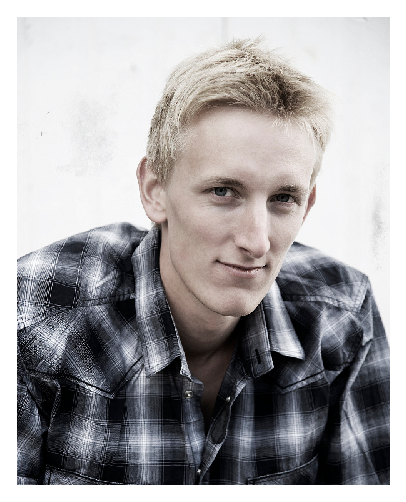
\includegraphics[width=1in,height=1.25in,clip,keepaspectratio]{bio/jo_inge.eps}}]{Jo Inge Buskenes}
received the B.Sc. degree in electrical engineering from Gj\o{}vik College University, Norway, in 2007, and the M.Sc. degree in instrumentation for particle physics from the University of Oslo, Norway, in 2010. He is currently pursuing the Ph.D. degree in image reconstruction and technology at the University of Oslo.

His industry experience includes the European Organization for Nuclear Research (CERN), Geneva, Switzerland (2007-2008), and the Norwegian Defence Research Establishment, Kjeller, Norway (2009). He has lectured in digital signal processing at the Gj\o{}vik College University (2009), and at the University of Oslo (2010-2013). His research interests include adaptive beamforming, digital image reconstruction, high performance computing, intelligent detector design and open source software.
\end{IEEEbiography}
% 
\begin{IEEEbiography}[{\includegraphics[width=1in,height=1.25in,clip,keepaspectratio]{bio/jon_petter.eps}}]{Jon Petter \AA{}sen}
(S'12) was born in Porsgrunn, Norway in 1986. He received the B.Sc. and M.Sc. degree in computer science from the University of Oslo, Norway, in 2010. He is currently pursuing his Ph.D. degree in medical ultrasound technology at the Norwegian University of Science and Technology (NTNU) Medical Imaging Lab (MI-Lab), Trondheim, Norway. His research interests include adaptive ultrasound processing techniques and acceleration of ultrasound algorithms using Graphics Processing Units (GPUs). 
\end{IEEEbiography}
% 
\begin{IEEEbiography}[{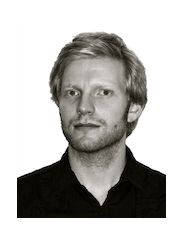
\includegraphics[width=1in,height=1.25in,clip,keepaspectratio]{bio/carl-inge.eps}}]{Carl-Inge Colombo Nilsen}
(S'06-M'10) received the M.Sc. and Ph.d. degrees in computer science from the University of Oslo, Norway, in 2005 and 2010. He is currently working at the University of Oslo as a postdoctoral research fellow. His research interests include signal and array processing for ultrasound imaging and other acoustical applications.
\end{IEEEbiography}
% 
\begin{IEEEbiography}[{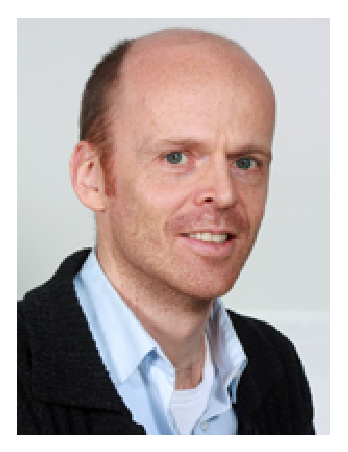
\includegraphics[width=1in,height=1.25in,clip,keepaspectratio]{bio/andreas.eps}}]{Andreas Austeng}
was born in Oslo, Norway, in 1970. He received the M.Sc. degree in physics in 1996 and the Ph.D. degree in computer science in 2001, both from the University of Oslo. Since 2001, he has been working at the Department of Informatics, University of Oslo, first as a postdoctoral research fellow and currently as an associate professor. His research interests include signal and array processing for acoustical imaging.
\end{IEEEbiography}


% 
% IMAGE METRICS
%
% - Point spread function (res via main lobe width, SAS gain via PDF height)
% - Constrast measures
%
% ACR = cL/2
% C = (s+n)/n ratio
% - 
% WHO's needing processing power
% - Centre for Maritime Research and Experimentation


\vfill 

\end{document}


